% ****** Start of file apssamp.tex ******
%
%   This file is part of the APS files in the REVTeX 4.1 distribution.
%   Version 4.1r of REVTeX, August 2010
%
%   Copyright (c) 2009, 2010 The American Physical Society.
%
%   See the REVTeX 4 README file for restrictions and more information.
%
% TeX'ing this file requires that you have AMS-LaTeX 2.0 installed
% as well as the rest of the prerequisites for REVTeX 4.1
%
% See the REVTeX 4 README file
% It also requires running BibTeX. The commands are as follows:
%
%  1)  latex apssamp.tex
%  2)  bibtex apssamp
%  3)  latex apssamp.tex
%  4)  latex apssamp.tex
%
\documentclass[%
% reprint,
%superscriptaddress,
%groupedaddress,
%unsortedaddress,
%runinaddress,
%frontmatterverbose, 
preprint,
%showpacs,preprintnumbers,
%nofootinbib,
%nobibnotes,
bibnotes,
% amsmath,amssymb,
% aps,
%pra,
%prb,	
%rmp,
%prstab,
%prstper,
%floatfix,
]{revtex4-1}

\usepackage{graphicx}% Include figure files
\usepackage{dcolumn}% Align table columns on decimal point
\usepackage{bm}% bold math
%\usepackage{hyperref}% add hypertext capabilities
%\usepackage[mathlines]{lineno}% Enable numbering of text and display math
%\linenumbers\relax % Commence numbering lines

%\usepackage[showframe,%Uncomment any one of the following lines to test 
%%scale=0.7, marginratio={1:1, 2:3}, ignoreall,% default settings
%%text={7in,10in},centering,
%%margin=1.5in,
%%total={6.5in,8.75in}, top=1.2in, left=0.9in, includefoot,
%%height=10in,a5paper,hmargin={3cm,0.8in},
%]{geometry}

\begin{document}

%\preprint{APS/123-QED}
%\begin{titlepage}

\includegraphics[width= 40mm]{aleph-logo.jpg}
\title{Proposal for Two-Particle Correlation Analyses with Belle Data}% Force line breaks with \\
%\thanks{A footnote to the article title}%

\author{Bibek Pandit}%
 \email{bibek@mit.edu}
\author{Anthony Badea}%
 \email{badea@mit.edu}
\author{Gian Michele Innocenti}%
 \email{ginnocen@mit.edu }
\author{Yen-Jie Lee}
 \email{yenjie@mit.edu}
 \affiliation{Massachusetts Institute of Technology}%
% \altaffiliation[Also at ]{Physics Department, XYZ University.}%Lines break automatically or can be forced with \\

%\collaboration{BELLE Collaboration}%\noaffiliation

\date{\today}% It is always \today, today,
             %  but any date may be explicitly specified

\begin{abstract}
Two-particle correlations in high-energy collisions provide valuable information for characterizing Quantum Chromodynamics and have been studied previously for a broad range of collision energies in proton-proton (pp), proton-nucleus (pA), and nucleus-nucleus (AA) collisions. In AA collisions, a significant long-range angular correlation between particles was observed. The common interpretation of the results based on the hydrodynamics calculations was that a thermalized system was created in the AA collisions. Recently, similar correlation signals were observed in high particle multiplicity pp and pA collisions. The physical origin of the phenomenon is not yet fully understood. Due to the complexity of the hadron-hadron collisions, possible initial state correlations of the partons, such as those arise from color-glass condensate, could complicate the interpretation of the pp and pA data. Studies of high multiplicity $e^+e^-$ collision, where the initial kinematics of the collisions are well-controlled, could bring significant insights about the observed phenomenon. This paper proposes measurements of two-particle angular correlations of charged hadrons produced in $e^+e^-$ collisions, as a function of charged hadron multiplicity with the Belle detector. These measurements will enable a direct comparison between $e^+e^-$, pp, pA and AA collisions for the first time. Preliminary results from Belle open data are also presented.
\end{abstract}

\pacs{Valid PACS appear here}% PACS, the Physics and Astronomy
                             % Classification Scheme.
%\keywords{Suggested keywords}%Use showkeys class option if keyword
                              %display desired
\maketitle

%\tableofcontents

%%% Introduction %%%
\section{Introduction}

This paper proposes measurements of two-particle angular correlations of charged hadrons produced in $e^+e^-$ collisions as a function of charged hadron multiplicity using 730 $pb^{-1}$ of archived data collected between 91 and 209 GeV with the ALEPH detector at LEP are presented.  Two-particle correlations in high-energy collisions provide valuable information for characterizing Quantum Chromodynamics and have been studied previously for a broad range of collision energies in proton-proton (pp)~\cite{Khachatryan:2010gv}, proton-nucleus (pA)~\cite{CMS:2012qk,Abelev:2012ola,Aad:2012gla}, and nucleus-nucleus (AA)~\cite{Aamodt:2010pa,Chatrchyan:2012wg} collisions. Such measurements can elucidate the underlying mechanism of particle production and reveal possible collective effects resulting from the high particle densities accessible in these collisions.

Studies of two-particle angular correlations are typically performed using two-dimensional $\Delta\eta-\Delta\phi$ correlation functions, where $\Delta\phi$ is the difference in the azimuthal angle $\phi$ between the two particles and $\Delta\eta$ is the difference in pseudorapidity $\eta = -\ln(\tan(\theta/2))$. The polar angle $\theta$ is defined relative to the counterclockwise hadron beam direction.

Of particular interest in studies of collective effects is the long-range (large $|\Delta\eta|$) structure of the two-particle correlation functions. In this region, the function is less susceptible to other known sources of correlations such as resonance decays and fragmentation function of energetic jets. Measurements in high-energy AA collisions have shown significant modification of the long-range structure compared with minimum-bias pp collisions, over a very wide range of collision energies~\cite{Back:2004je,Arsene:2004fa,Adcox:2004mh,Adams:2005dq}. The long-range correlations are commonly interpreted as a consequence of the hydrodynamical flow of the produced strongly interacting medium~\cite{Ollitrault:1992bk} and usually characterized by the Fourier components of the azimuthal particle distributions. The extraction of the second and third Fourier components, usually referred to as elliptic and triangular flow, is of great interest because it is closely related to initial collision geometry and its fluctuation~\cite{Alver:2010gr}. Those measurements allow the extraction of the fundamental transport properties of the medium using hydrodynamic models.

Recently, measurements in pp~\cite{Khachatryan:2010gv} and pPb collisions~\cite{CMS:2012qk,Abelev:2012ola,Aad:2012gla} have revealed the emergence of long-range, near-side ($\Delta\phi\sim 0$) correlations in the selection of collisions with very high number of final state particles. This ``ridge-like'' correlation has inspired a large variety of theoretical models~\cite{Bzdak:2013zma,Dusling:2015gta}. The physical origin of the phenomenon is not yet fully understood. Moreover, it was found that the elliptic flow signal exists even at the lowest nucleon-nucleon center-of-mass energy of 7.7 GeV in AA collisions at the Relativistic Heavy Ion Collider~\cite{Adamczyk:2012ku}. 

Due to the complexity of the hadron-hadron collisions, possible initial state correlations of the partons, such as those arise from color-glass condensate~\cite{Gelis:2010nm, Dusling:2013qoz}, could complicate the interpretation of the pp and pA data. Studies of high multiplicity $e^+e^-$ collision, where the initial kinematics of the collisions are well-controlled, could bring significant insights about the observed phenomenon. These measurements will also enable a direct comparison between different collision systems for the first time. The studies of ridge signal in $e^+e^-$ collisions will bring significant impact to the field of relativistic heavy ion collisions, either change completely the interpretation of the ridge in pp, pA and AA collisions if a significant signal is observed, or serve as an important reference for the final state effect observed in high multiplicity hadron-hadron scatterings if no long-range correlation signal was detected. 

With the archived data, the correlation functions are studied over a broad range of pseudorapidity $\eta$ (rapidity $y$) and azimuthal angle $\phi$ with respect to the electron-positron beam axis and the event thrust axis. 


%%% Analysis %%%
\section{Two-Particle Correlation Function}

In this analysis with Belle open data, identified protons, pions and kaons with transverse momentum between 0.1 and 4.0 GeV/$c$ 
are selected for the correlation function analysis. High multiplicity events are sampled using the total number of selected proton, 
pions and kaons (hadron multiplicity $N$) in each event. The first step in extracting the correlation function was to divide the sample 
into bins in the hadron multiplicity. For each hadron multiplicity class, ``trigger" particles are defined as charged particles originating 
from primary vertex in the selected transverse momentum range (0.1 and 4.0 GeV/$c$). The number of trigger particles in the event is denoted
by $N_{trig}$. Particle pairs are then formed by associating every trigger particle with the remaining charged primary particles in the 
same $p_{\rm T}$ interval as the trigger particle. The per-trigger-particle associated yield is defined as:
\begin{eqnarray}
\label{eq:associatedyield}
\frac{1}{N_{\rm trig}}\frac{\rm d^2N^{pair}}{d\Delta\eta  \rm d\Delta\phi}= B(0,0) \times \frac{S(\Delta\eta, \Delta\phi)}{B(\Delta\eta, \Delta\phi)}
\end{eqnarray}
where $\Delta\eta$ and $\Delta\phi$ are the differences in $\eta$ and $\phi$ of the pair. The signal distribution, $S(\Delta\eta, \Delta\phi)$, 
is the per-trigger-particle yield of particle pairs in the same event: 
\begin{eqnarray}
\label{eq:S}
S(\Delta\eta,\Delta\phi) = \frac{1}{N_{trig}}\frac{\rm d^2 N^{\rm same}}{\rm d\Delta\eta \rm d\Delta\phi}
\end{eqnarray}
The mixed-event background distribution, used to account for random combinatorial background, is defined as 
\begin{eqnarray}
\label{eq:B}
B(\Delta\eta,\Delta\phi) = \frac{1}{N_{trig}}\frac{\rm d^2 N^{\rm mix}}{\rm d\Delta\eta \rm d\Delta\phi}
\end{eqnarray}
and is constructing by pairing the trigger particles from two random events in the same hadron multiplicity interval.
The symbol $N^{mix}$ denotes the number of pairs taken from the mixed event, while $B(0,0)$ represents the 
mixed-event associated yield for both particles of the pair going in the same direction and thus having full pair acceptance. Therefore, 
the ratio $B(0,0)/B(\Delta\eta,\Delta\phi)$ represents the pair-acceptance correction factor used to derive the corrected per-trigger-particle
associated yield distribution.  The signal and background distributions are first calculated for each event and then averaged over all the events 
within the track multiplicity class.


%%% Results %%%
\section{Preliminary Results from Belle Open Data}

Figure~\ref{fig:multPID} shows the multiplicity distribution of identified particles (pions, kaons and proton) obtained after 
applying the selection on the particle transverse momentum (0.1 $<p_{\rm T}<$ 4.0 GeV/$c$). 
The dominant contribution to the total multiplicity is coming as expected from pions.
In Fig.~\ref{fig:multHadron}, the charged hadron multiplicity distribution $N$ is shown: the largest raw particle multiplicity observed in these events is about 70 before corrections for tracking efficiency, fakes and multiple reconstruction rate. 

\begin{figure}[!htb]
\begin{center}
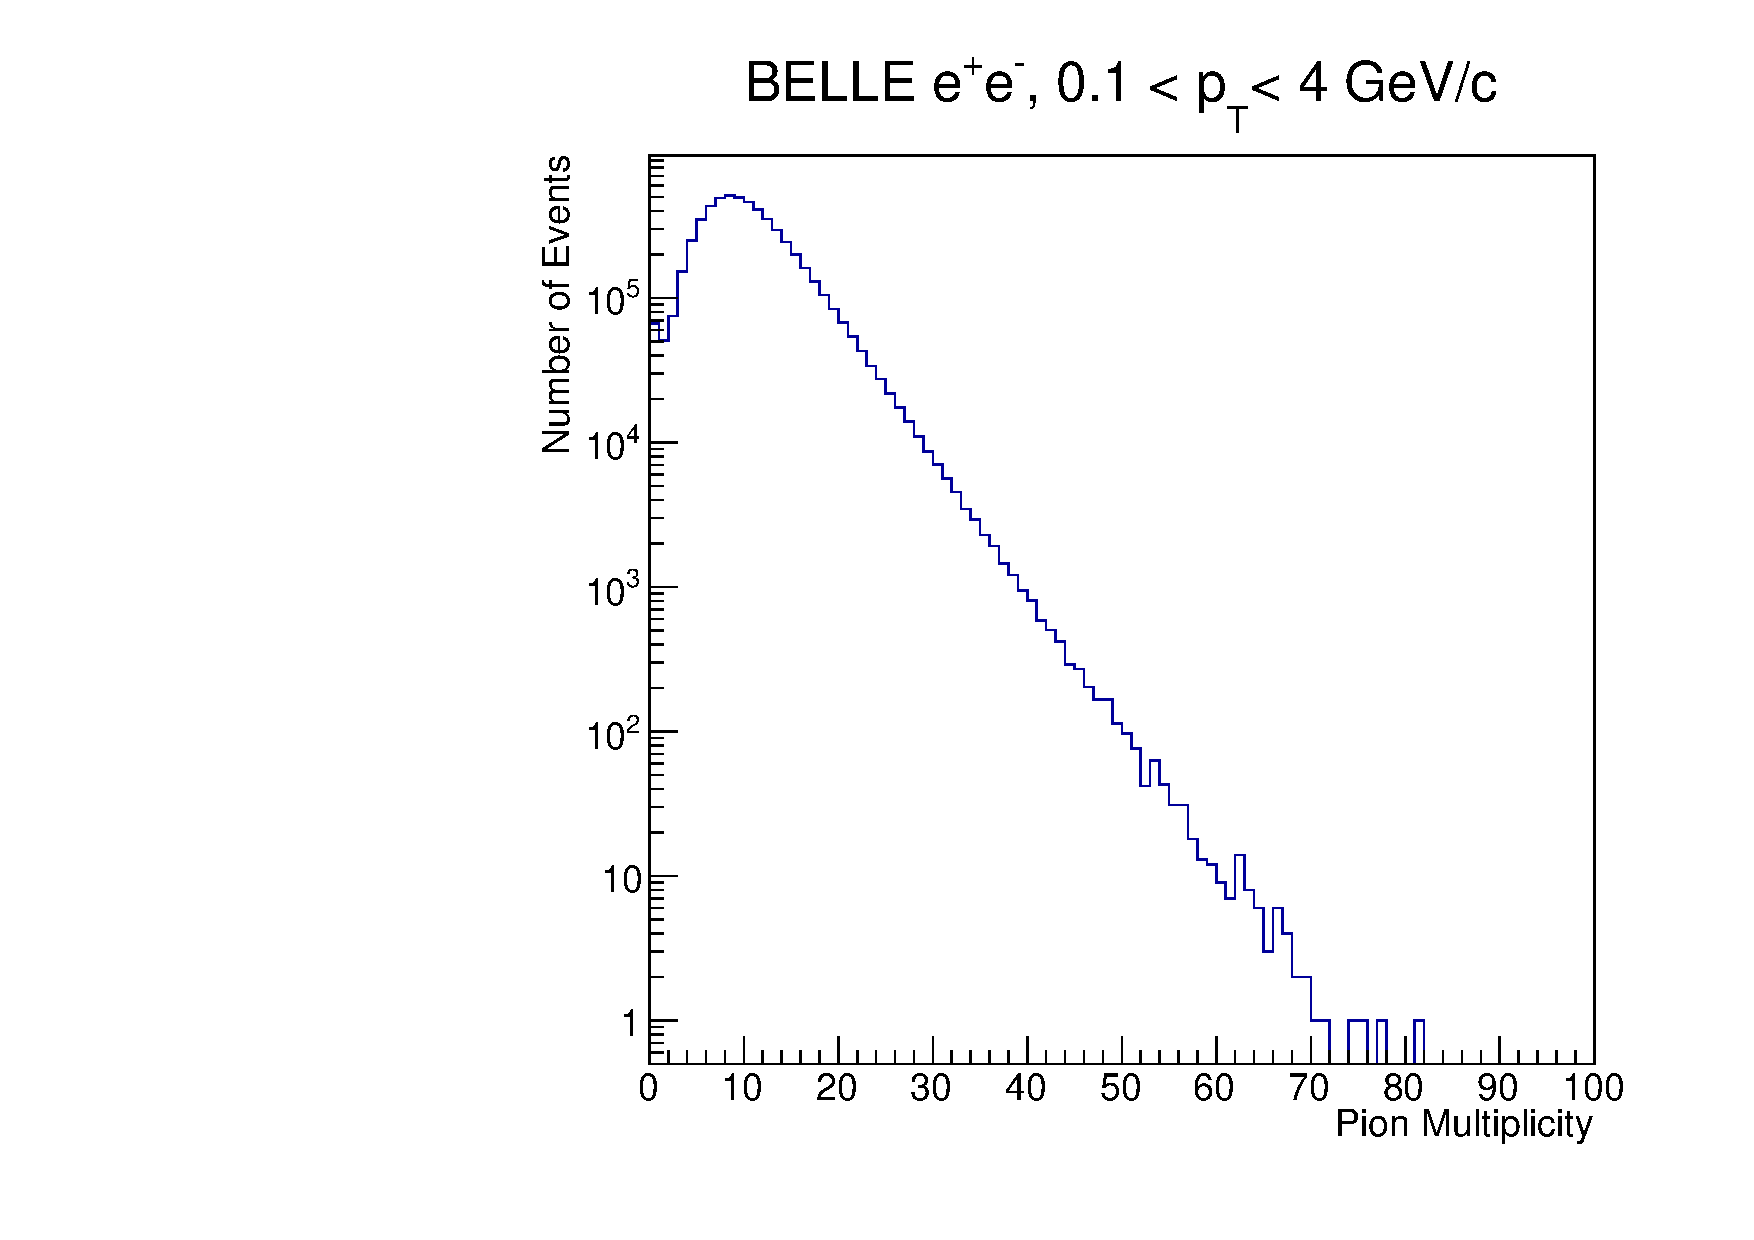
\includegraphics[width=.32\textwidth]{figures/pion_mult.pdf}
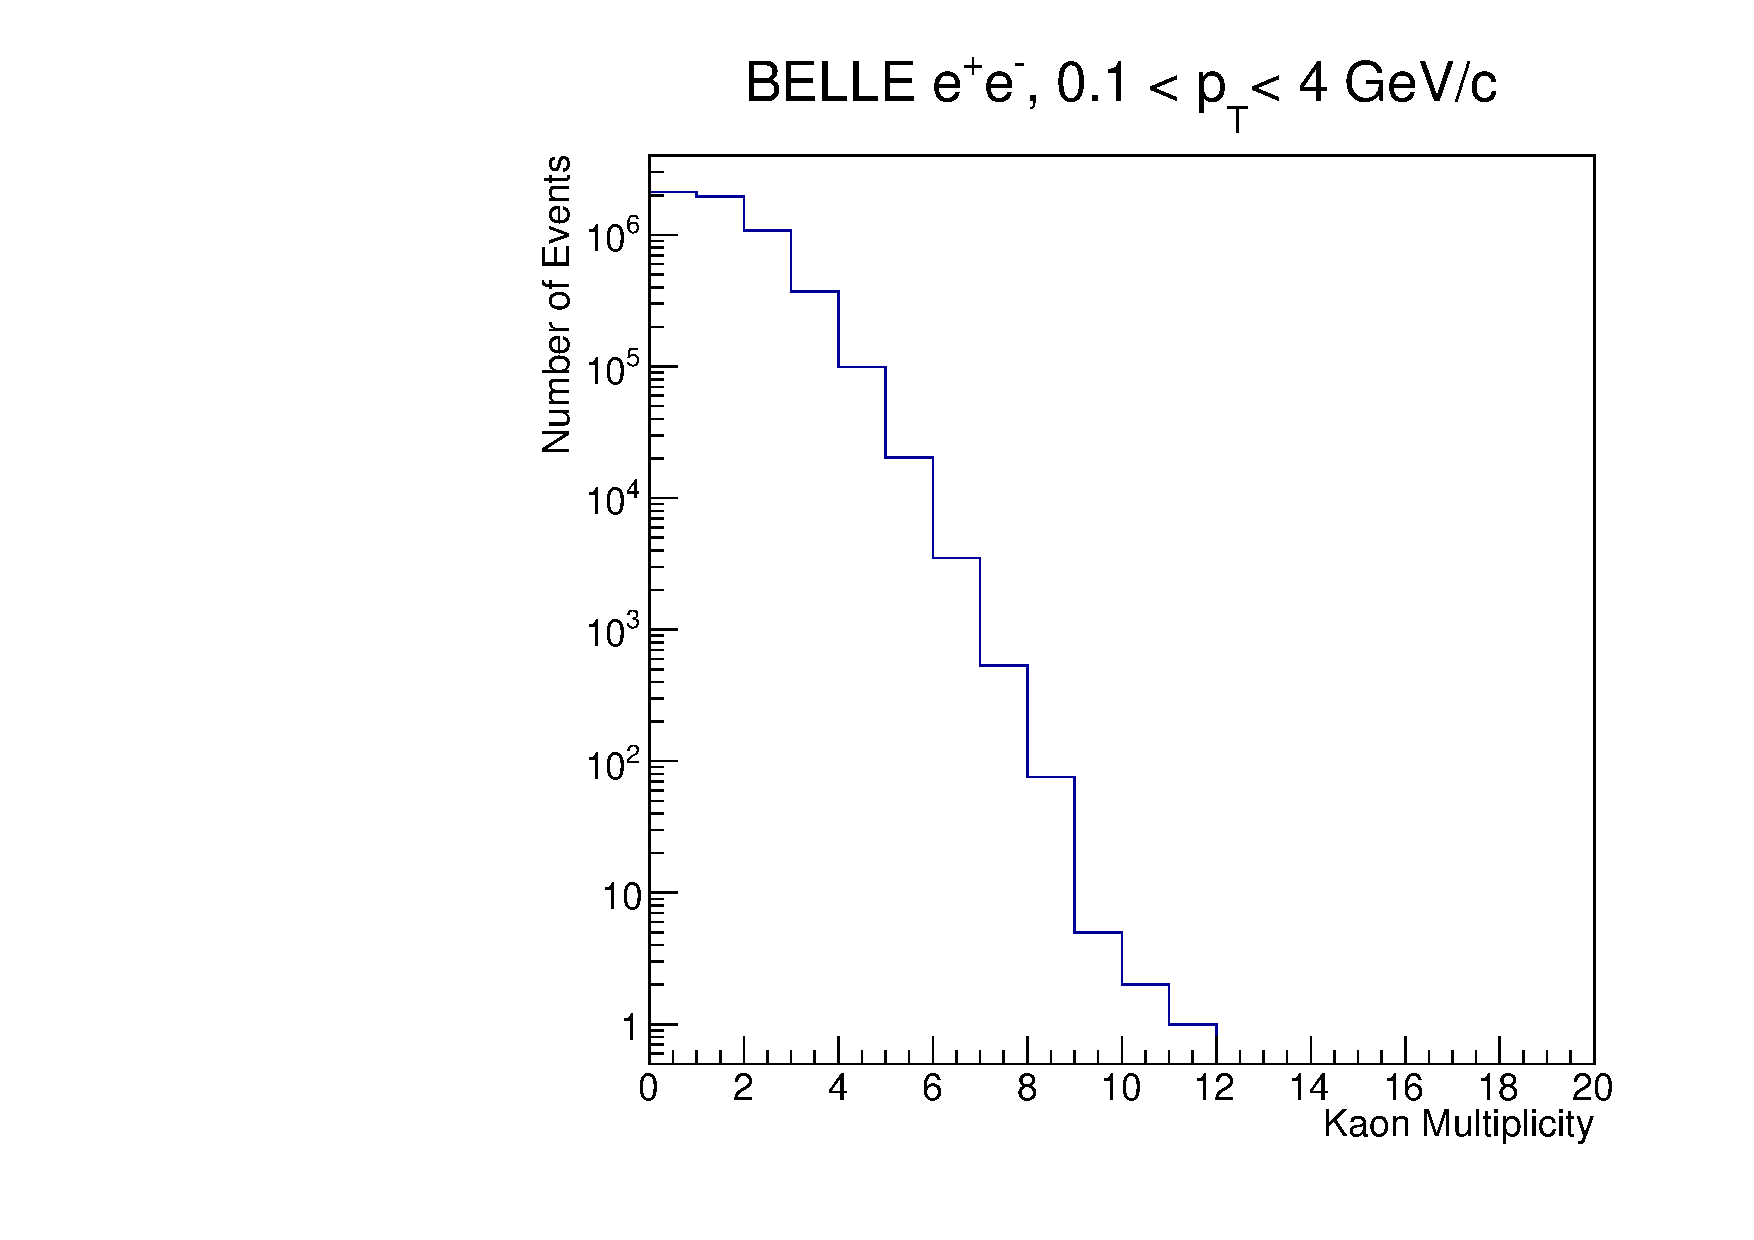
\includegraphics[width=.32\textwidth]{figures/kaon_mult.pdf}
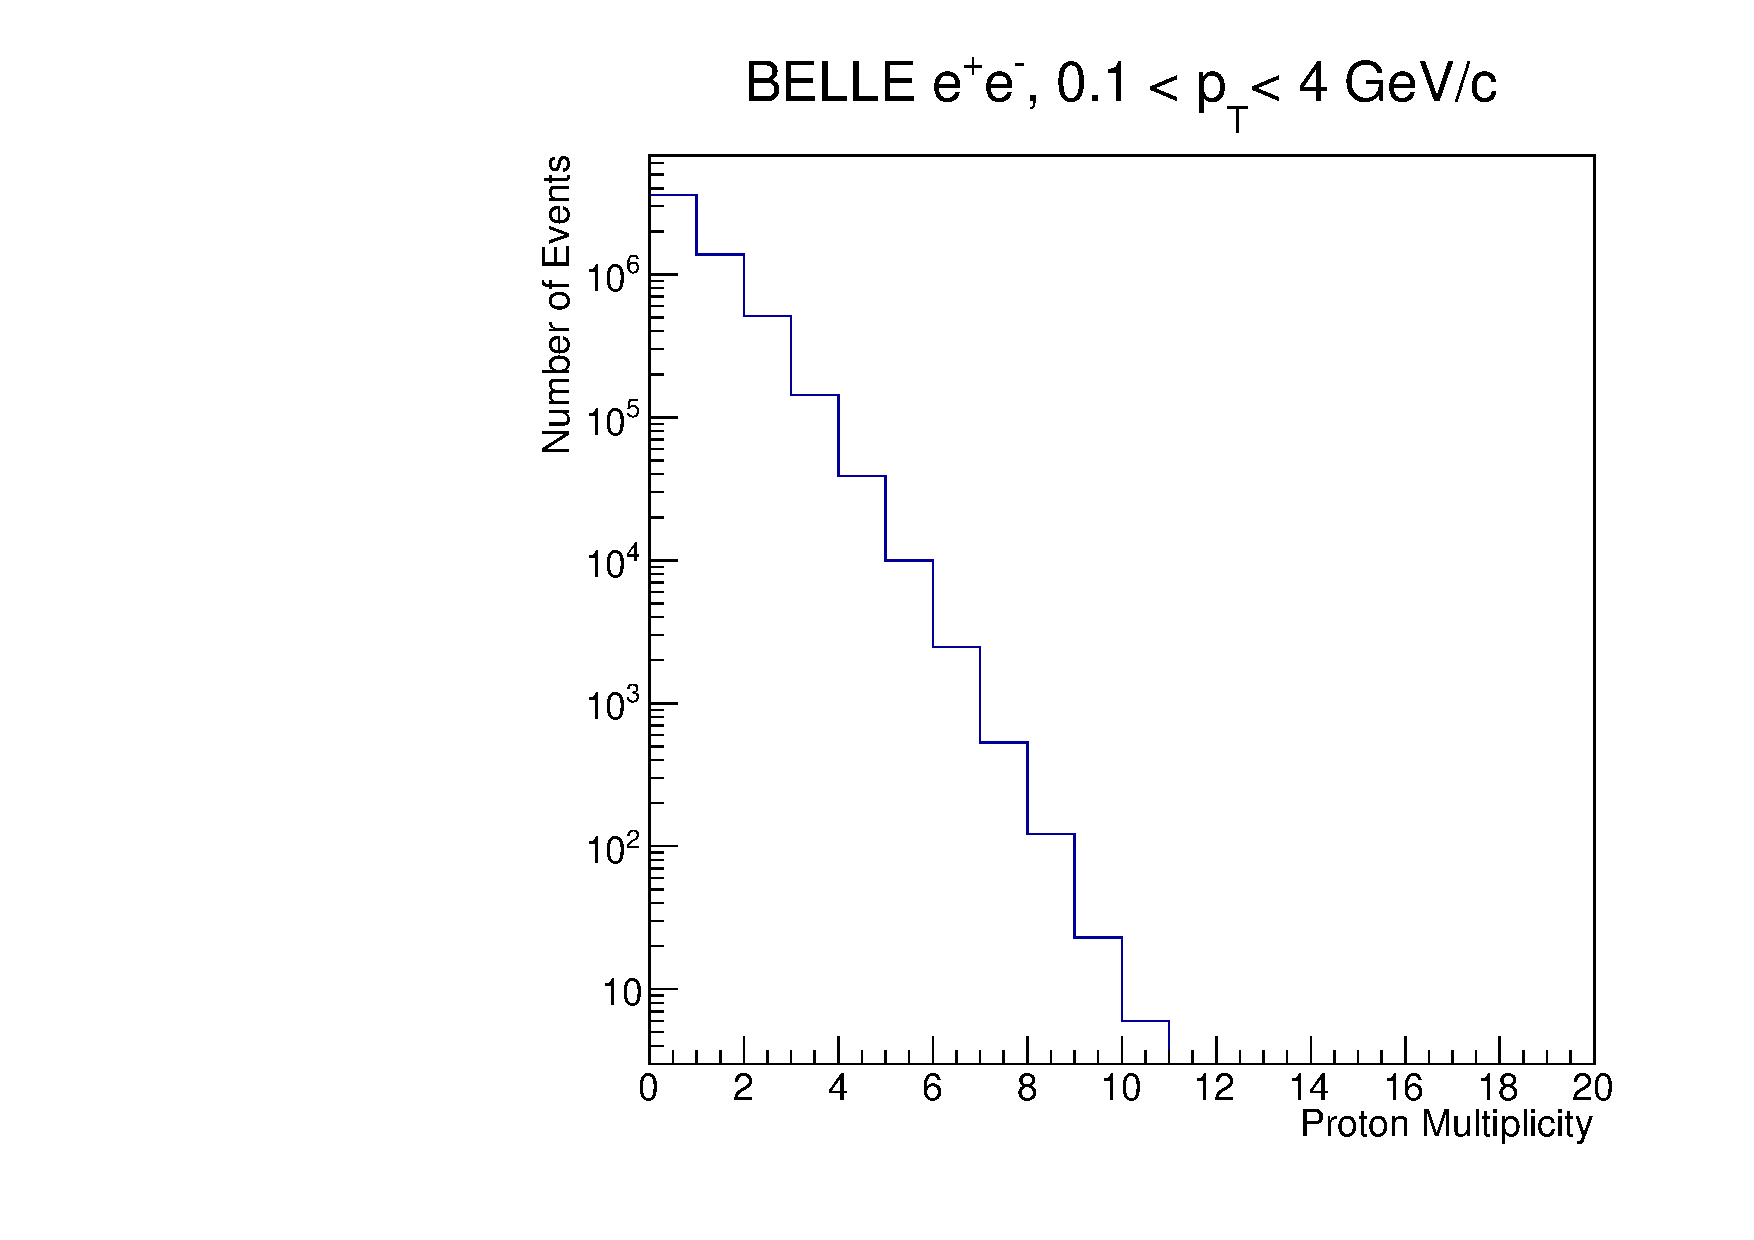
\includegraphics[width=.32\textwidth]{figures/proton_mult.pdf}
\caption{Uncorrected multiplicity distributions of pions (left), kaons (middle), protons (right) for  particles in the range  0.1 $<p_{\rm T}<$ 4.0 GeV/$c$ in $e^{+}e^{-}$ collisions. }
\label{fig:multPID} 
\end{center}
\end{figure}

\begin{figure}[!htb]
\begin{center}
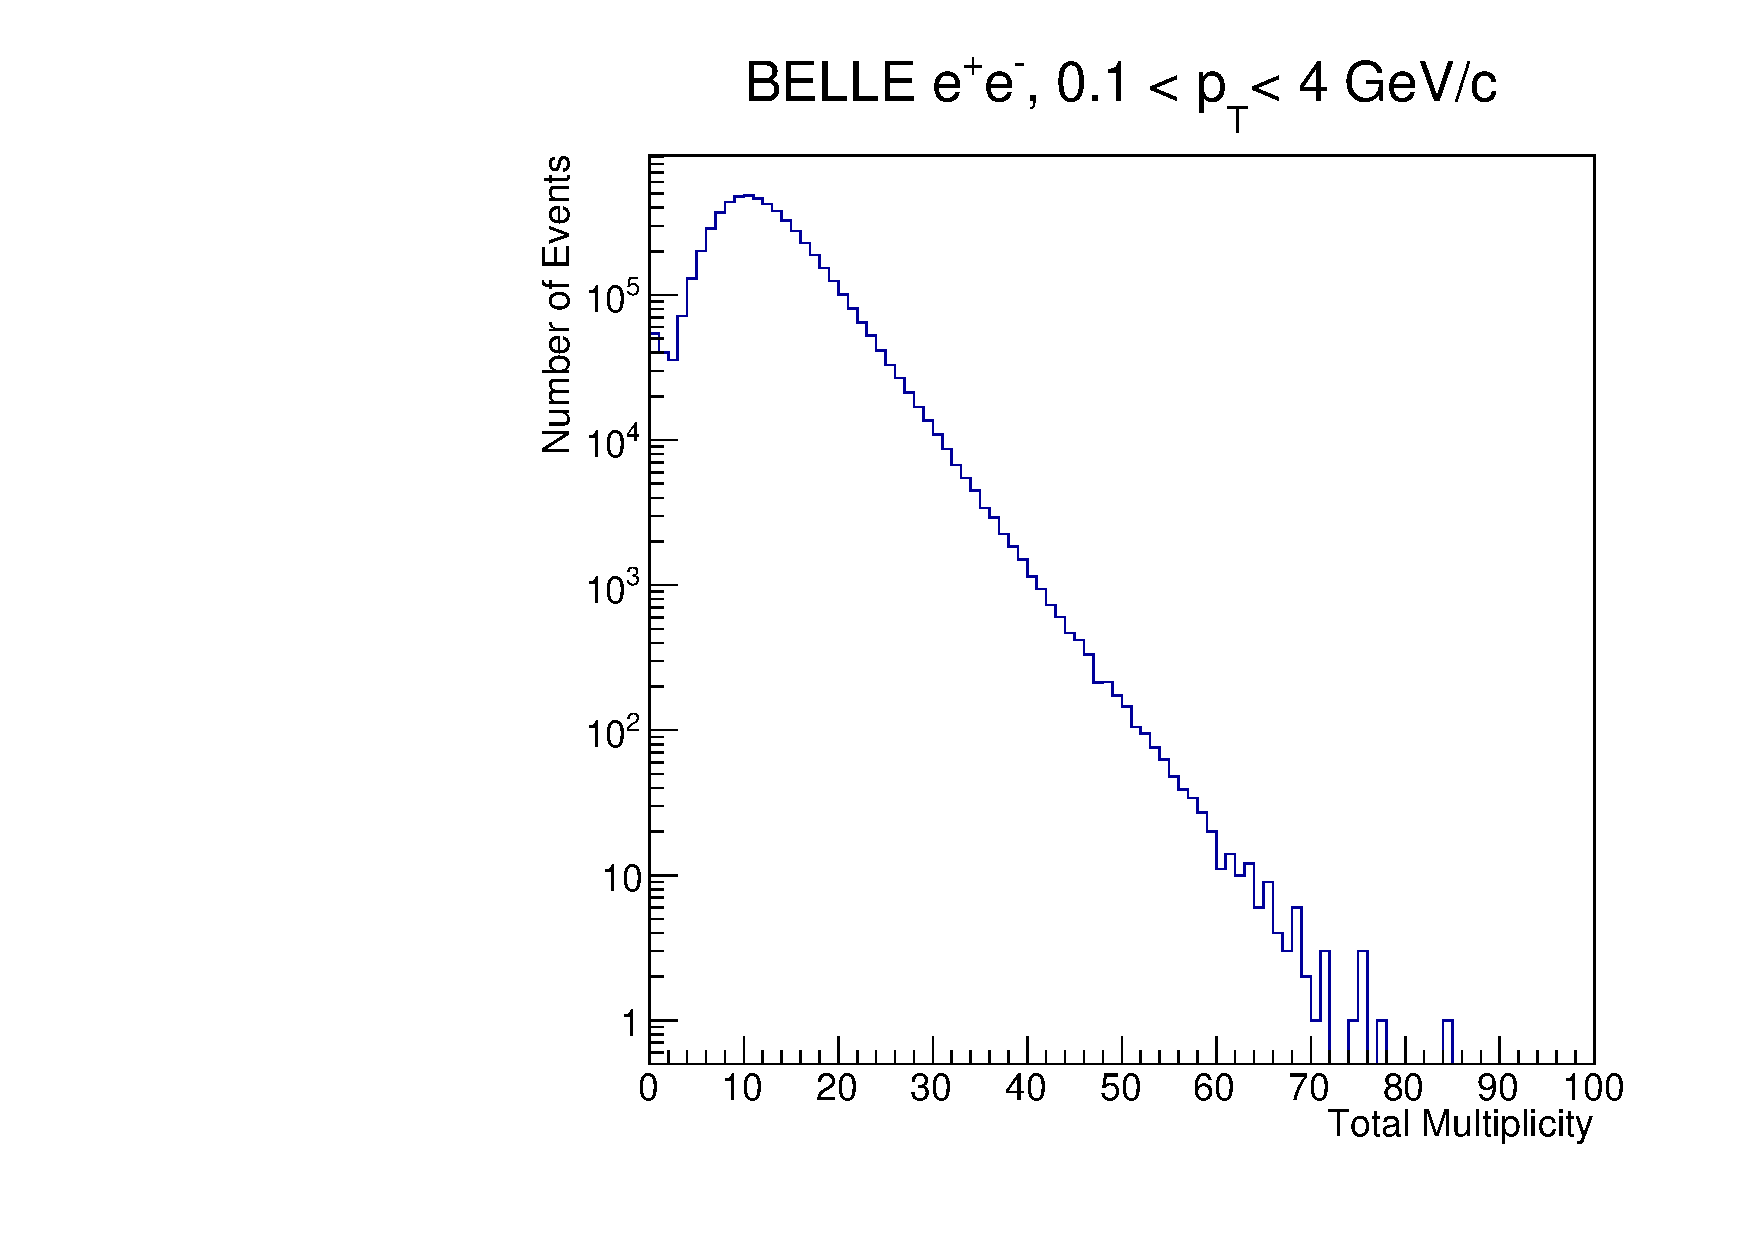
\includegraphics[width=.45\textwidth]{figures/total_mult.pdf}
\caption{Multiplicity distribution of charged hadrons (protons, kaons and pions) for  particles in the range  0.1 $<p_{\rm T}<$ 4.0 GeV/$c$ in $e^{+}e^{-}$ collisions. }
\label{fig:multHadron} 
\end{center}
\end{figure}

In this proposal we present the first study of two particle correlations with $e^{+}e^{-}$ with the Belle experiment using open data.
In Fig.~\ref{fig:ridgeBelle} we compare the two-particle correlation functions for events with low (N$>$20) and high multiplicity(N$>40$). 
In the low-multiplicity result, the dominant features are the correlation peak near $(\Delta\eta,\Delta\phi)=(0,0)$ for pairs of particles originating from the same jet 
and the elongated structure at $\Delta\phi\sim\pi$ for pairs of particles from back-to-back jets. To better illustrate the full correlation structure, the jet peak has been truncated.
Moving from low-multiplicity to high-multiplicity selection, the same-side jet peak and back-to-back correlation structures can be observed. 
However, in addition, a hint of ``ridge"-like structure is visible at $\Delta\phi \sim$0. This ridge has characteristics which are similar to the structures
observed in high multiplicity pp and pPb collisions at $\sqrt{s_{NN}}$ and in AA collisions over a wide range of energies.

To check if a long-range ridge structure exists, one-dimensional distributions in $\Delta\phi$ are obtained by integrating over different $|\Delta\eta|$ interval, 0$<|\Delta \eta|<$1 (left) and 
2$<|\Delta \eta|<$3 (right). In the left side plot, we can clearly identify the near side peak at $\Delta\phi=$0 and the back-to-back peak at $\Delta\phi=\pi$. At large pseudorapidities, 
a hint of signal at $\Delta\phi=0$ seems to confirm the observation of a long-range correlation structure. This preliminary observation motivates a detailed study with the highest 
statistics data taken by the Belle collaboration. 

\begin{figure}[!htb]
\begin{center}
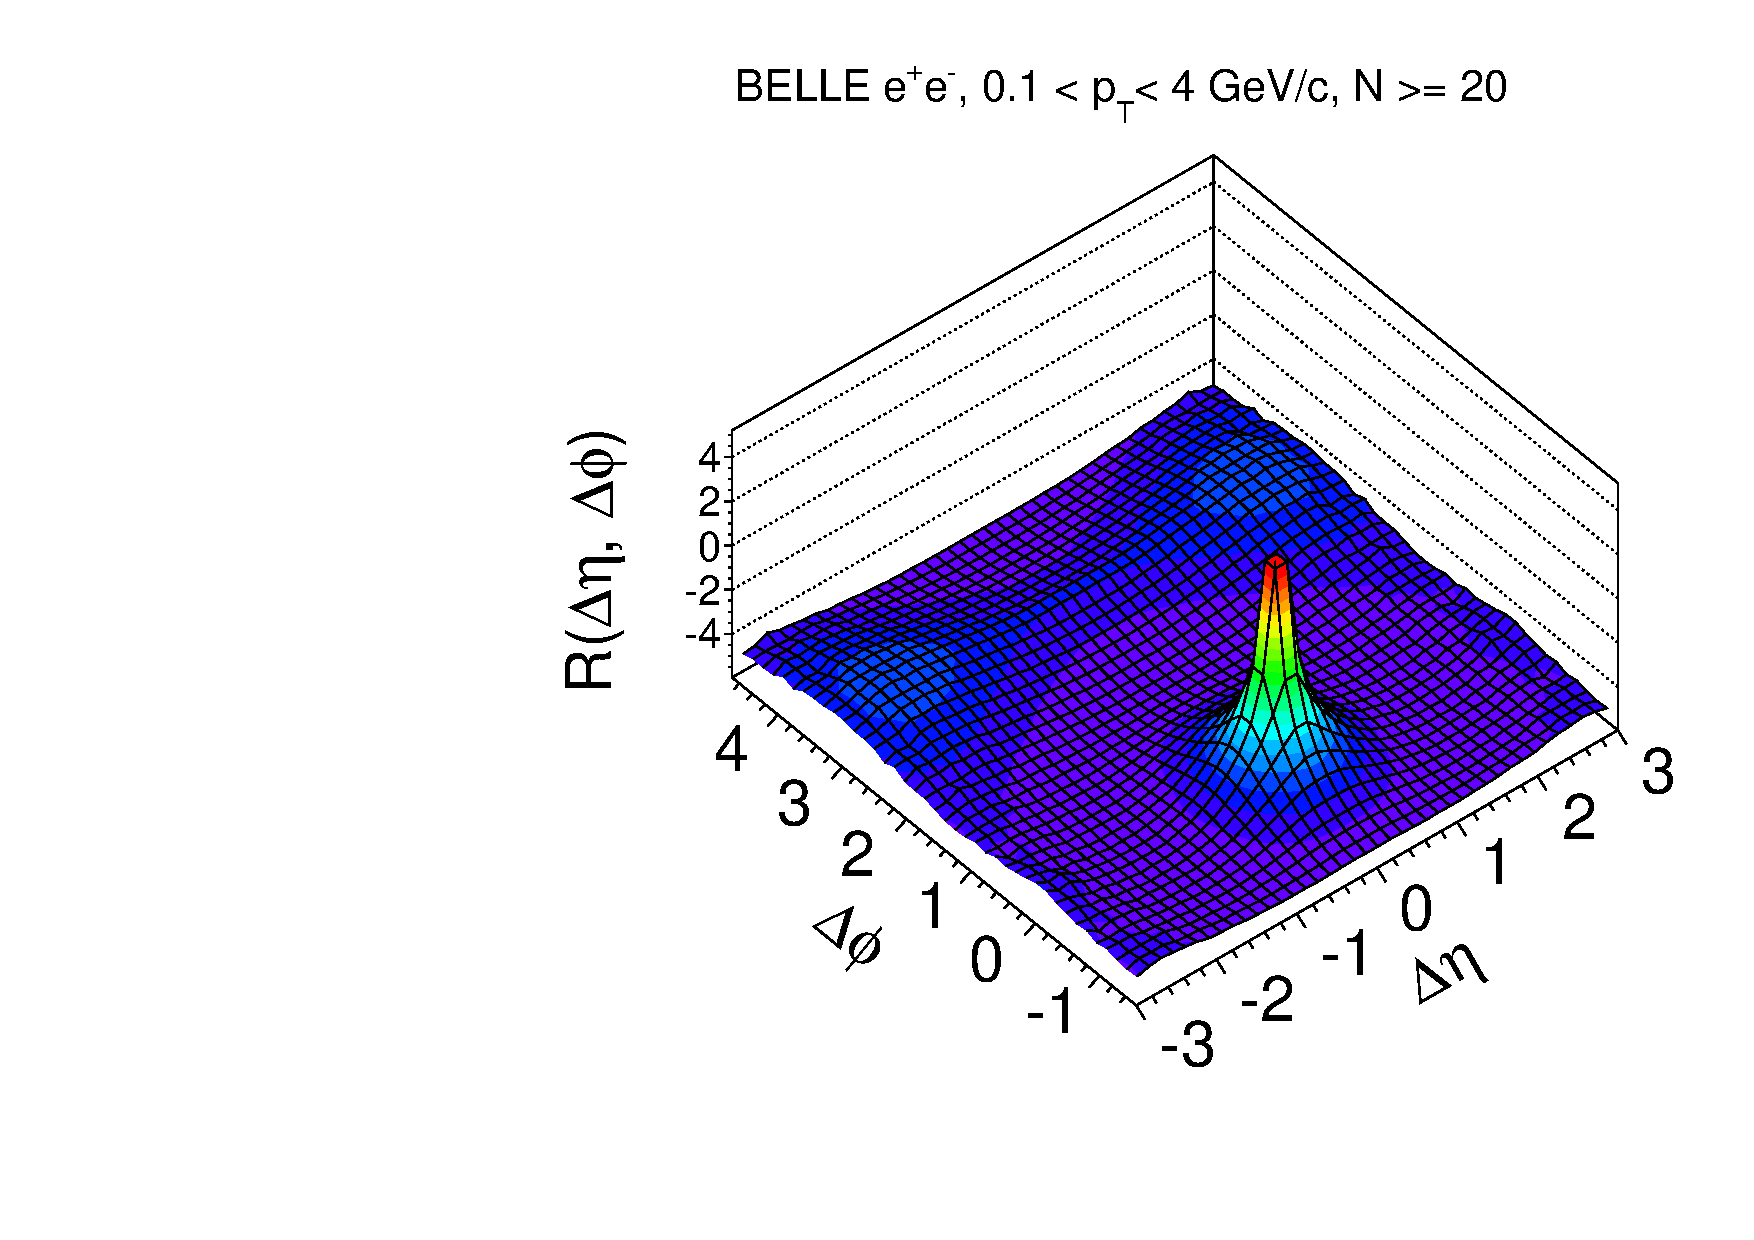
\includegraphics[width=.45\textwidth]{figures/canvasRidgeBelleMult20CutHigh0.pdf}
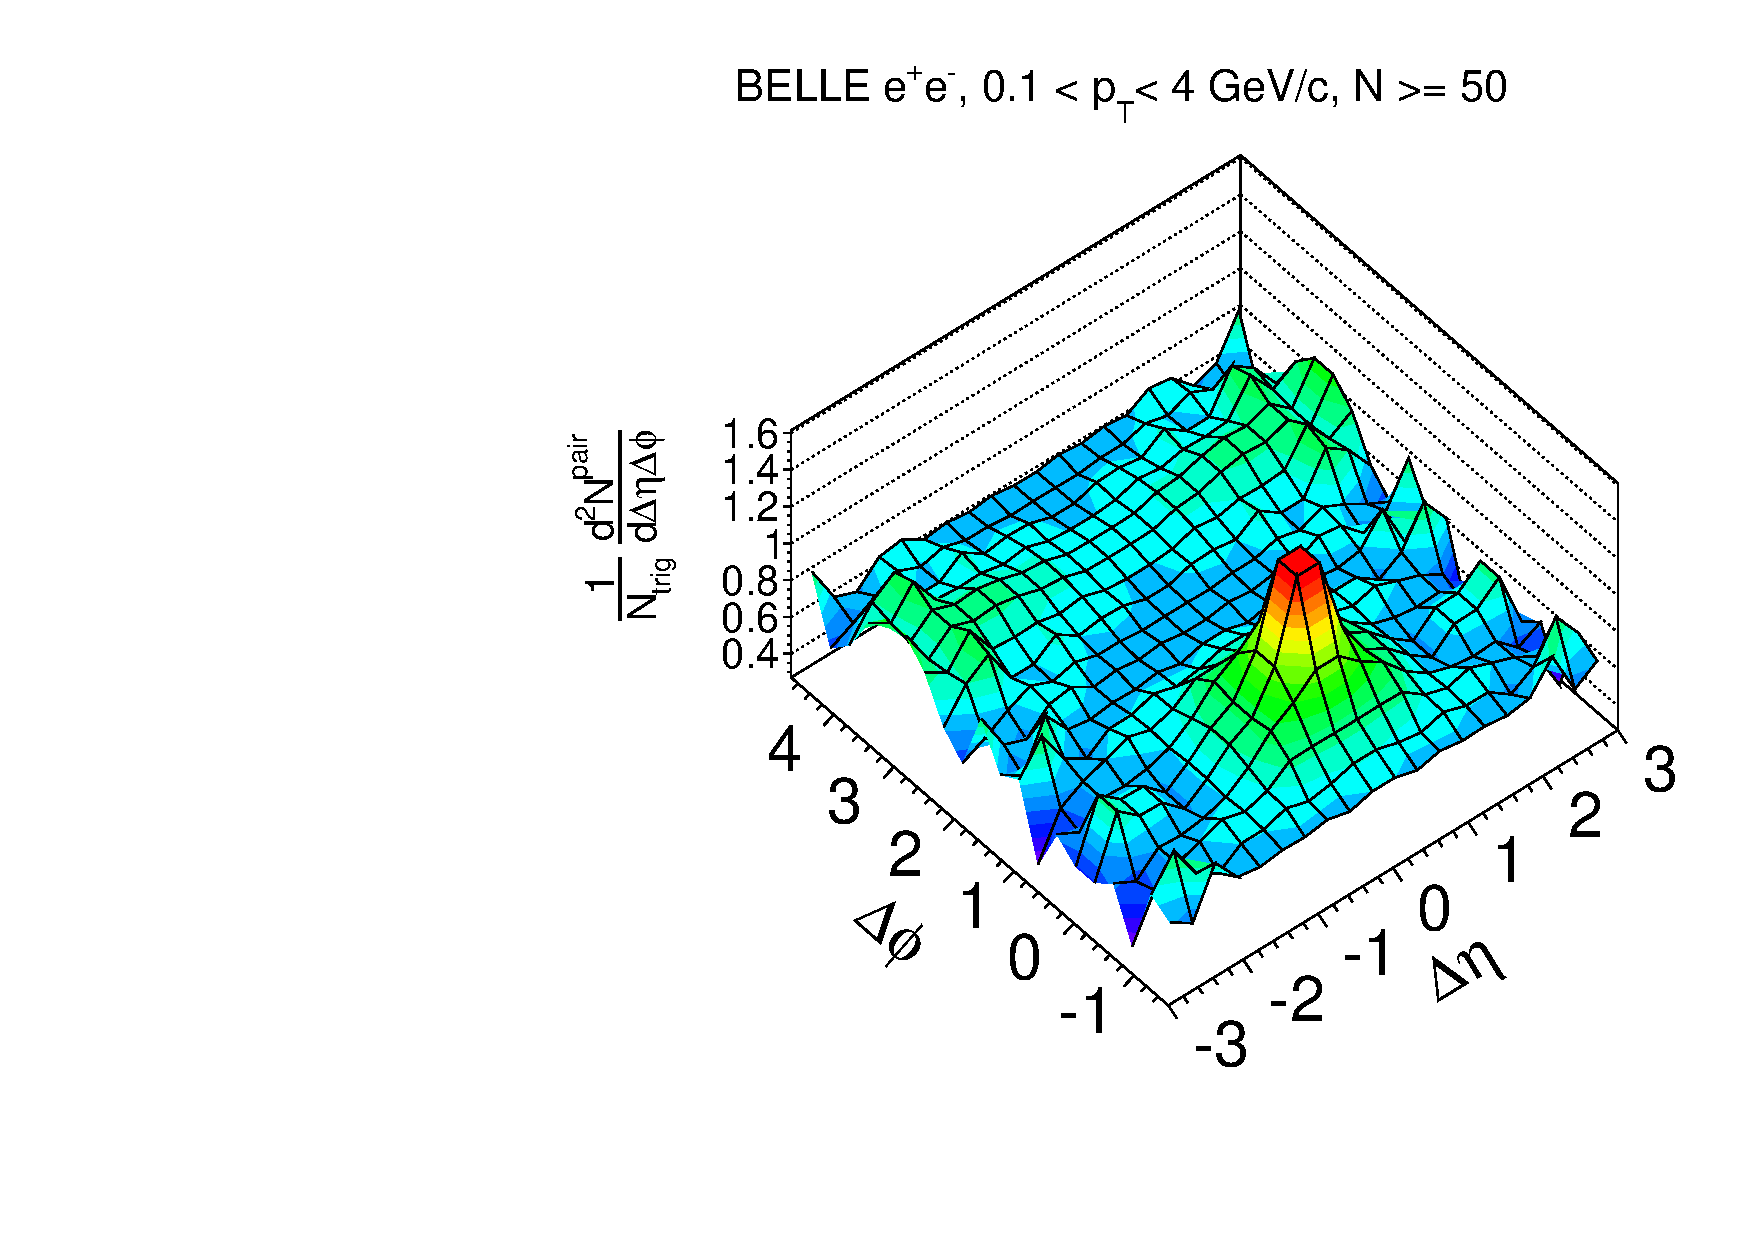
\includegraphics[width=.45\textwidth]{figures/canvasRidgeBelleMult50CutHigh0.pdf}
\caption{Two-particle correlation functions versus $\Delta\eta$ and $\Delta\phi$ in $e^{+}e^{-}$ collisions for events with particle multiplicity $>$ 20 (left) and  $>$ 50 (right).}
\label{fig:ridgeBelle} 
\end{center}
\end{figure}

\begin{figure}[!htb]
\begin{center}
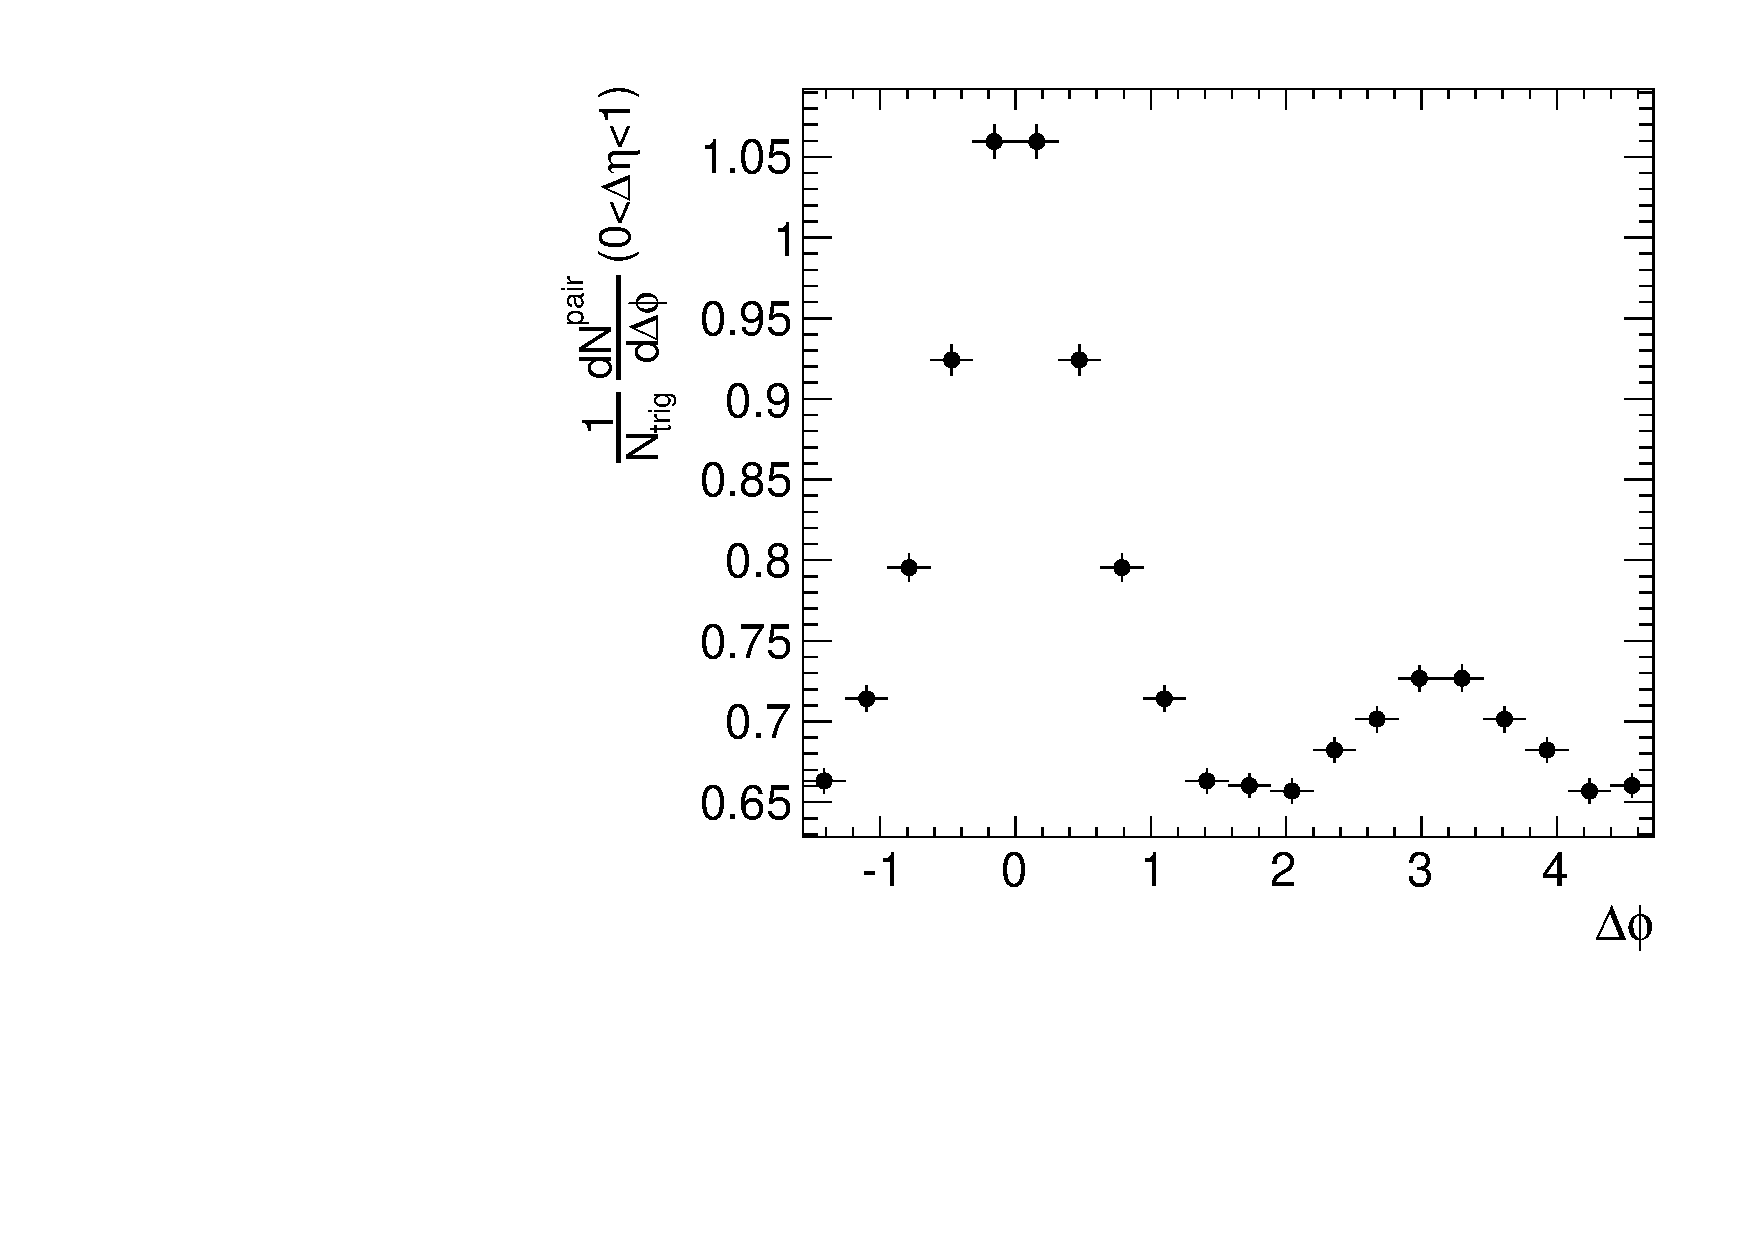
\includegraphics[width=.45\textwidth]{figures/canvasProjection_isBelle1_mult50_eta01.pdf}
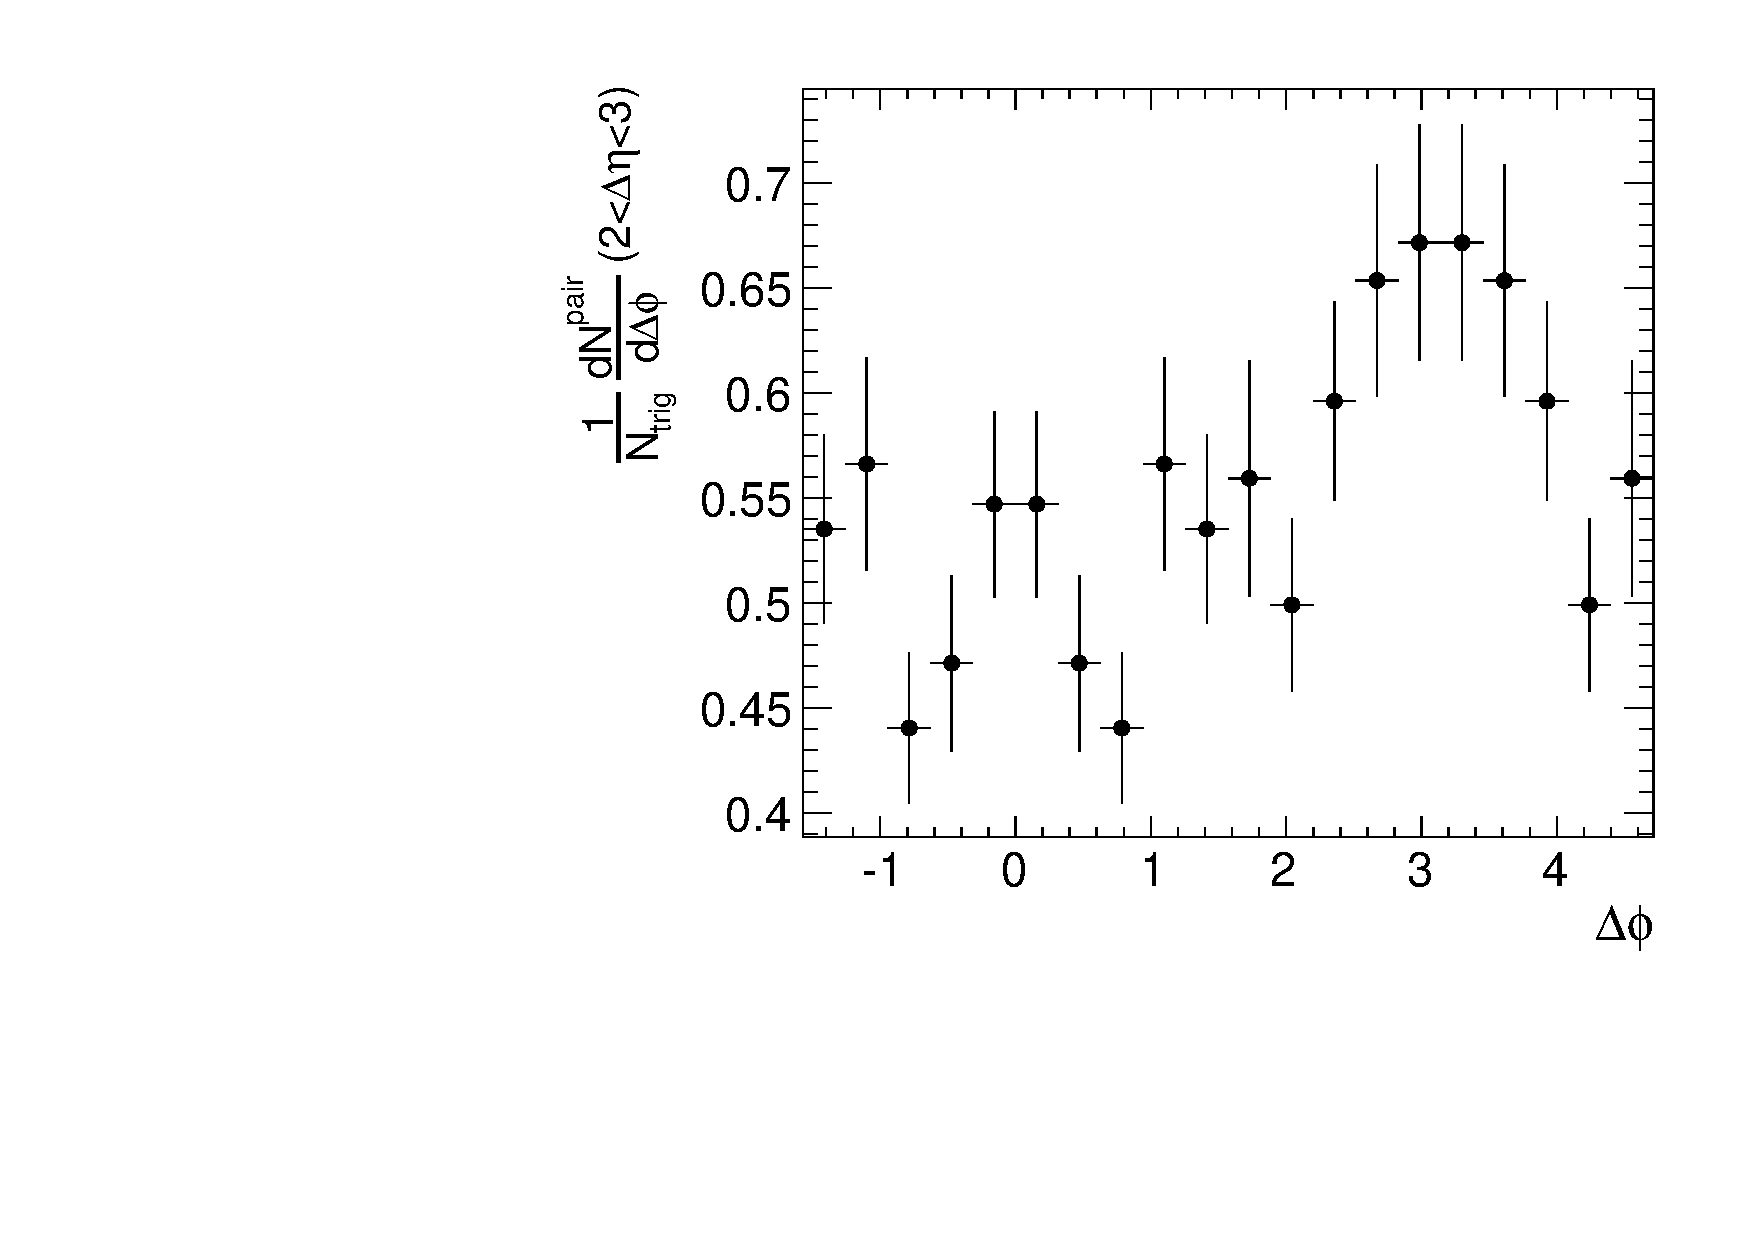
\includegraphics[width=.45\textwidth]{figures/canvasProjection_isBelle1_mult50_eta23.pdf}
\caption{Two-particle correlation functions as a function of  $\Delta\phi$ in $e^{+}e^{-}$ in the pseudorapidity ranges 0$<\Delta \eta<$1 (left) and 2$<\Delta \eta<$3 (right).}
\label{fig:ProjectionMult50} 
\end{center}
\end{figure}



%%% Summary %%%
\section{Summary}

The Belle open data has been used to measure angular correlations between
two charged particles. A hint of long-range ridge-like structure at the
near-side ($\Delta\phi\sim 0$) was seen in the Belle data. The observation of
long-range near-side ridge like correlation (or the non-observation) with the full Belle dataset will bring significant impact to the interpretation of the pp, pA and AA data.



\bibliography{main}{}
\bibliographystyle{lucas_unsrt}
\end{document}
%
% ****** End of file apssamp.tex ******
